%==============================================================================
% Sjabloon poster bachproef
%==============================================================================
% Gebaseerd op document class `a0poster' door Gerlinde Kettl en Matthias Weiser
% Aangepast voor gebruik aan HOGENT door Jens Buysse en Bert Van Vreckem

\documentclass[a0,portrait]{hogent-poster}

% Info over de opleiding
\course{Bachelorproef}
\studyprogramme{toegepaste informatica}
\academicyear{2023-2024}
\institution{Hogeschool Gent, Valentin Vaerwyckweg 1, 9000 Gent}

% Info over de bachelorproef
\title{Onderzoek naar pentesting binnen specifieke webomgevingen}
\author{Levi Van Achter}
\email{levi.vanachter@student.hogent.be}
\supervisor{Benjamin Vertonghen }
\cosupervisor{Stijn D'Hollander (Sinergio)}

% Indien ingevuld, wordt deze informatie toegevoegd aan het einde van de
% abstract. Zet in commentaar als je dit niet wilt.
\specialisation{Mobile & Enterprise developmen}
\keywords{Penetratietesten, Webapplicaties, Beveiliging, Ethical Hacking, Cybersecurity}
%\projectrepo{https://github.com/user/repo}

\begin{document}

\maketitle

\begin{abstract}
  Dit onderzoek richt zich specifiek op penetratietesten binnen een webomgeving, waarbij de focus ligt op het
  identificeren en beveiligen van kwetsbaarheden in webapplicaties. Het omvat een grondige verkenning van
  methodologieën en technieken die worden toegepast bij het testen van de beveiliging van webapplicaties. Het
  onderzoek analyseert populaire webgerichte aanvalsvectoren zoals SQL-injecties, cross-site scripting (XSS) en
  cross-site request forgery (CSRF). Daarnaast wordt een vergelijkende studie uitgevoerd om de effectiviteit van
  de testen op meten bij 3 verschillende we applicaties
\end{abstract}

\begin{multicols}{2} % This is how many columns your poster will be broken into, a portrait poster is generally split into 2 columns

\section{Introductie}

Cybersecurity is een cruciaal, maar vaak onderbelicht aspect binnen softwareontwikkeling. Deze bachelorproef onderzoekt 
de effectiviteit en gebruiksvriendelijkheid van verschillende penetratietesttools in drie specifieke webomgevingen: een 
WordPress-omgeving zonder beveiligingsplugins, een WordPress-omgeving met beveiligingsplugins, en een Laravel-applicatie.

Door gestructureerde penetratietests met tools zoals Burp Suite, OWASP ZAP en Metasploit, worden kwetsbaarheden in elke 
omgeving geanalyseerd en de gebruiksvriendelijkheid van deze tools beoordeeld. De resultaten tonen aan dat de WordPress-
omgeving zonder beveiligingsplugins het meest kwetsbaar is, terwijl de Laravel-applicatie de hoogste weerstand biedt 
dankzij geavanceerde beveiligingsmaatregelen.

Daarnaast blijken Burp Suite en OWASP ZAP zeer gebruiksvriendelijk te zijn, terwijl Metasploit uitblinkt in diepgaande 
testmogelijkheden. Dit onderzoek benadrukt de noodzaak van effectieve beveiligingsstrategieën en biedt praktische 
aanbevelingen voor de selectie en implementatie van penetratietesttools in softwareprojecten.

\section{Experimenten}

In dit hoofdstuk worden de experimenten beschreven die zijn uitgevoerd met drie penetratietesttools: Burp Suite, OWASP 
ZAP, en Metasploit. Deze tools zijn toegepast op een WordPress-omgeving met beveiligingsplugins. Voor Burp Suite zijn 
daarnaast testen uitgevoerd in drie verschillende webomgevingen: een WordPress-omgeving zonder beveiligingsplugins, 
een WordPress-omgeving met beveiligingsplugins, en een Laravel-applicatie.

De eerste reeks experimenten betrof het gebruik van Burp Suite in de WordPress-omgeving met beveiligingsplugins. 
Hierbij werden twee specifieke aanvallen uitgevoerd: een brute force attack en een SQL-injectie. Deze tests waren 
gericht op het identificeren van kwetsbaarheden ondanks de aanwezigheid van beveiligingsplugins.

OWASP ZAP werd eveneens ingezet in de WordPress-omgeving met beveiligingsplugins, waarbij ook brute force attacks 
en SQL-injecties werden uitgevoerd. Het doel was om te beoordelen hoe effectief de beveiligingsplugins deze aanvallen 
konden blokkeren en om de gebruiksvriendelijkheid van de tool te evalueren.

Metasploit werd gebruikt om diepgaandere aanvalsscenario's te simuleren in dezelfde omgeving. Hierbij werd eveneens een
brute force attack uitgevoerd om te bepalen hoe goed de beveiligingsplugins in staat waren om deze  aanvallen 
te weerstaan.

ook werd er telkens gekeken naar de gebruiksvriendelijkheid van de tools dit werd bepaald aan de hand van hoeveel 
tijd het in beslag nam voor er getest kon worden. Ook werd dit bepaald op basis van hoeveel kennis er nodig was om 
de tool te gebruiken.

Daarnaast werd Burp Suite afzonderlijk getest in drie verschillende webomgevingen. In de WordPress-omgeving zonder 
beveiligingsplugins werden brute force attacks uitgevoerd om te zien hoe kwetsbaar de site was zonder 
extra beveiligingsmaatregelen. In de WordPress-omgeving met beveiligingsplugins werd dezelfde aanval uitgevoerd om 
de effectiviteit van de plugins te beoordelen. Ten slotte werd Burp Suite gebruikt om de Laravel-applicatie te testen met 
brute force attacks, waarbij werd gekeken naar de ingebouwde beveiligingsmaatregelen van het framework.

Door deze gestructureerde aanpak kon de effectiviteit en gebruiksvriendelijkheid van de penetratietesttools in 
verschillende webomgevingen grondig worden geëvalueerd.

\begin{center}
  \captionsetup{type=figure}
  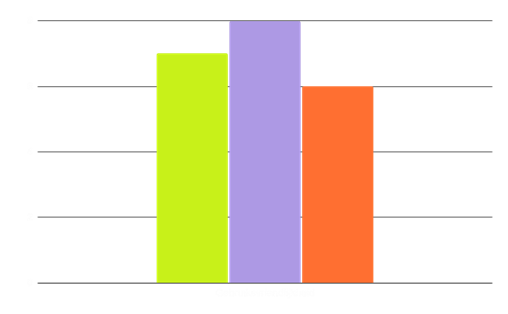
\includegraphics[width=1.0\linewidth]{tools_2}
  \captionof{figure}{gebruikvriendelijkheid per tool op 10}
\end{center}

Let er wel op dat dit tot problemen met bladschikking kan leiden.

\section{Conclusies}
De prestaties van Burp Suite, Metasploit en OWASP ZAP varieerden niet veel bij het identificeren van kwetsbaarheden in de 
drie specifieke webomgevingen. Bij brute force-aanvallen op een WordPress-omgeving beveiligd met de Wordfence-plugin 
slaagden geen van de tools erin het wachtwoord te kraken vanwege de limiet van inlogpogingen. De gebruiksvriendelijkheid 
varieerde: Burp Suite scoorde 7/10, Metasploit 6/10, en OWASP ZAP 8/10

In een WordPress-omgeving zonder beveiligingsplugins werden door de tools meerdere kwetsbaarheden blootgelegd. De tools 
konden het wachtwoord in 90\% van de gevallen binnen 3 minuten kraken, wat de hoge kwetsbaarheid van onbeveiligde 
WordPress-sites benadrukt. Beveiligingsplugins zoals Wordfence reduceerden het aantal succesvolle brute force-aanvallen 
drastisch. De Laravel-applicatie toonde robuuste beveiliging, waarbij geen enkele tool het wachtwoord kon kraken.

Beveiligingsplugins verbeterden de detectiecapaciteiten van de tools aanzienlijk. Ze beperkten het aantal inlogpogingen, 
vergrendelden accounts na overschrijding van de limiet, en stuurden real-time alerts bij verdachte activiteiten. OWASP ZAP 
en de betaalde versie van Burp Suite detecteerden bekende kwetsbaarheden met hoge efficiëntie.

\section{Toekomstig onderzoek}

Voor toekomstig onderzoek zijn er verschillende interessante mogelijkheden om de bevindingen van deze studie verder uit te 
breiden. Een belangrijk aspect dat nog nader onderzocht kan worden, is het gebruik van de Burp Suite Professional Edition. 
Deze versie biedt uitgebreidere functionaliteiten en diepgaandere analyseopties dan de Community Edition, waardoor een extra 
vergelijking kan worden gemaakt met andere penetratietesttools zoals Metasploit en OWASP ZAP.

Daarnaast kunnen toekomstige studies zich richten op het testen van nieuwe beveiligingsplugins en updates binnen de 
WordPress- en Laravel-omgevingen. Het is essentieel om te evalueren hoe deze verbeteringen de effectiviteit van bestaande 
beveiligingsmaatregelen beïnvloeden en of ze nieuwe kwetsbaarheden introduceren.
\end{multicols}
\end{document}